This section evaluates the performance of the cached profile implementation using modern benchmark suites. The goal is to provide indicators on the performance influence and try to analyze where this performance influence comes from. Since we try to decrease warmup time and decrease the number of deoptimizations 
\section{Setup}
\label{s:perf_setup}
To provide reliable and comparable results all tests were done on a single node of the Data Center Observatory provided by ETH \cite{ethdco}.
A node features 2 8-Core AMD Opteron 6212 CPUs running at 2600 MHz with 128 GB of DDR3 RAM and a solid state disk.
The node is running Fedora 19 and GCC 4.8.3. All JDK builds got created on the node itself.
\\\\
To compare performance the following benchmarks were used:
\begin{enumerate}
  \item \textbf{SPECjvm 2008:} A benchmark suite developed by Standard Performance Evaluation Corporation for measuring the performance of the Java Runtime Environment \cite{specjvm}.  I use version 2008 and I run a subset of 17 out of a total of 21 benchmarks. 4 are omitted due to incompatibility with openJDK 1.9.0.
  \\
  Once finished, SPECjvm prints out the number of operations per minute. This is used to compare the performance and higher is better.
  \item \textbf{Octane 2.0:} A benchmark developed by Google to measure the performance of JavaScript code found in large, real-world applications \cite{octane}. Octane runs on Nashorn, a JavaScript Engine on top of Hotspot. The version used is 2.0 and consists of 17 individual benchmarks of which 16 are used.
  \\
  Octane gives each benchmark a score reflecting the performance, the higher the score, the better the performance.
\end{enumerate}
The benchmarking process was automated using a number of self-written python scripts. The graphs in this chapter always show the arithmetic mean of 50 runs and the error bars display the 95\% confidence intervals.

\section{Benchmark performance}
\label{s:perf_benchmark}
The main goal of cached profiles is to improve the startup performance of the JVM. Having a rich profile from an earlier execution will allow the JIT compiler to use a highly optimized version right from the beginning.
We expect the modes to produce different results. The following list suggests reasons for these performance differences:
\begin{itemize}
  \item Some benchmarks might profit from compiling methods very early and therefore favor Mode 0.
  \item That could however result in many early compilations that overload the compilation queue resulting in worse performance. In this case Mode 1 will perform better than Mode 0.
  \item In case a cached profile can not be used (i.e. the limit of 10 deoptimizations was reached) the JVM needs to use freshly generated profiles. In case the thresholds were lowered (Mode 0) this compilation might have happened very early and only very incomplete profiles were available. This effect is less a problem when Mode 1 is used.
  \item Mode 2 keeps the steps of the original tiered compilation and is considered the most conservative mode. It puts the same load on the compile queue than the baseline version.
\end{itemize}
I will start by looking at SPECjvm since it offers ways to focus on the warmup. An individual description of each benchmark being used can be found in Appendix \ref{a:specjvm_benchmark}.
\subsection{SPECjvm warmup performance}
\label{s:perf_specjvm_warmup}
The longer a program is running the less impact a faster warmup has. Considering most benchmarks include a warmup phase which does not count towards the final score simply running the complete benchmark suite is not an option.
Instead I limited SPECjvm to 1 single operation which, depending on the benchmark take around 6 to 40 seconds.
Additionally, the JVM gets restarted between each single benchmark to prevent methods shared between benchmarks being compiled already.
\\\\
I run each benchmark with all cached profiling features disabled. This run is called the \textit{baseline} and displays the current openJDK 1.9.0 performance.    
\\\\ 
I then use a single benchmark run where I dump the profiles to disk. This run is not limited to a single operation and instead uses the default values of the benchmark. By default the benchmark is limited by time and runs for about 6 minutes. The idea is that these profiles include information that are usually not available during warmup and result in less deoptimizations and better code quality.
\\\\
These profiles are then used in 3 individual runs using the introduced \texttt{-XX:CacheProfiles} flag. Each run is using one of the 3 different CacheProfilesModes.
\begin{figure}[ht]
  \begin{center}
    \centering
    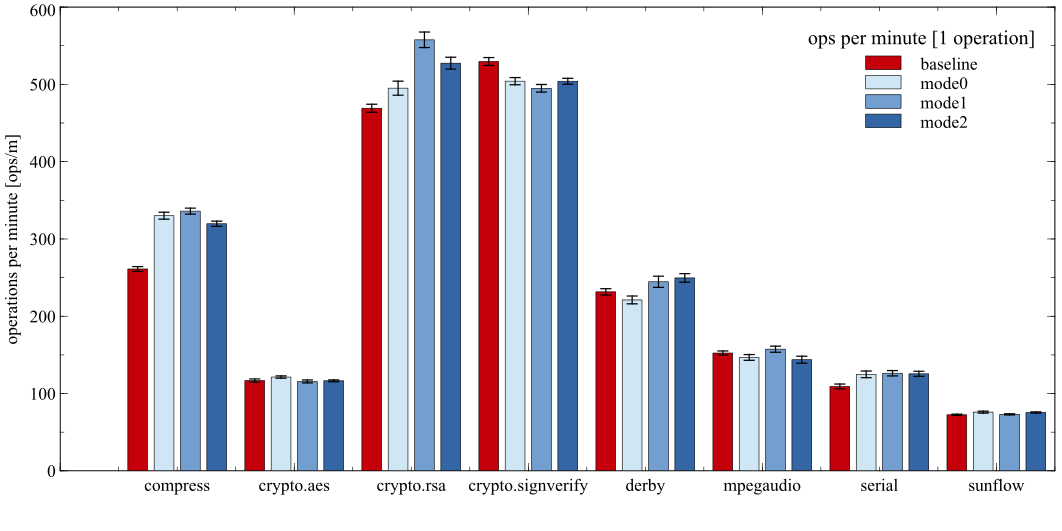
\includegraphics[width=1.0\textwidth]{figures/others_warmup.png}
    \caption{SPECjvm benchmarks on all different modes}
    \label{f:others_warmup}
  \end{center}
\end{figure}
\begin{figure}[ht]
  \begin{center}
    \centering
    \includegraphics[width=1.0\textwidth]{figures/scimark_warmup.png}
    \caption{SPECjvm scimark benchmarks on all different modes}
    \label{f:scimark_warmup}
  \end{center}
\end{figure}

\begin{figure}[ht]
  \begin{center}
    \centering
    \includegraphics[width=1.0\textwidth]{figures/all_warmup_variation.png}
    \caption{Relative performance from baseline for all SPECjvm benchmarks}
    \label{f:all_warmup_variation}
  \end{center}
\end{figure}
Figures \ref{f:others_warmup} and \ref{f:scimark_warmup} shows the number of operations per minute, measured for each benchmark individually. Note, that the operations per minute is not to be confused with the \textit{1 operation }of the benchmark itself.
Figure \ref{f:all_warmup_variation} summarizes the results by showing the relative performance compared to the baseline.
\\\\
The individual benchmarks show different effects on performance. Taking the average of all modes, we see a performance increase up to around 34\% in the compress benchmark (Mode 1) and a performance decrease of down to 20\% in scimark.sparse.large (Mode 0).
\\\\
Interestingly, the performance differences between the modes is not the same when comparing the individual benchmarks. For example in crypto.rsa Mode 0 clearly performs worst but in scimark.sparse.small it performs best.
JVM performance is known to be very hard to predict and it seems not to be different when cached profiles are used. On average the performance of the benchmark warmup is improved by 2.64\%, 3.37\%, and 2.67\% for Mode 0, Mode 1 and Mode 2.
\\\\
Between the three different modes there is no clear \textit{winner}. Each mode wins and looses in certain benchmarks against the others in terms of performance. However, in 12 out of 17 benchmarks at least one of the CacheProfileModes improves performance. 
\\\\
We will take a more detailed look at single benchmarks later in this chapter. 
\subsection{Octane performance}
\label{s:perf_octane}
Since the individual Octane benchmarks are rather short (most of them run for between 4 and 30 seconds) and there is no way to run a fixed number of iterations (without modifying the Octane source) we run the Octane benchmarks completely. We still split up the execution in the individual benchmarks to achieve many JVM restarts. The rest of the setup is identical to the SPECjvm run in Section \ref{s:perf_specjvm_warmup}.
\\\\
The absolute results are shown in Figure \ref{f:octane} and a relative comparison with the baseline in Figure \ref{f:octane_variation}.
Compared to SPECjvm the Octane performance is more scattered. The richards benchmark increases by around 50\% in Mode 0 while navierstockes decreases by around 25\% in Mode 1. In most benchmarks (9 out of 14) Mode 0 performs worst.
We assume this is related to the increased load of the compile queue and will therefore take a more detailed look at this in Section \ref{s:perf_compilequeue}. The performance of the two other modes is better in most benchmarks, but in total only 6 out of 14 benchmarks result in a performance improvement in at least one mode.

\begin{figure}[ht]
  \begin{center}
    \centering
    \includegraphics[width=1.0\textwidth]{figures/octane.png}
    \caption{Octane benchmarks on all different modes}
    \label{f:octane}
  \end{center}
\end{figure}

\begin{figure}[ht]
  \begin{center}
    \centering
    \includegraphics[width=1.0\textwidth]{figures/octane_variation.png}
    \caption{Relative performance from baseline for all Octane benchmarks}
    \label{f:octane_variation}
  \end{center}
\end{figure}
\section{Deoptimizations}
\label{s:perf_deoptimizations}
We are still eager to figure out where the performance increase and decrease come from.
We aim to lower the time needed for warmup by compiling methods earlier and or at lower tiers but also expect to decrease the number of deoptimizations by having more complete profiles early, which ideally results in better compiled code quality. To measure the total amount of deoptimizations we added a new compiler flag \texttt{-XX:+PrintDeoptimizationCount}.
The total number of deoptimizations of the SPECjvm benchmarks is shown in Figure \ref{f:others_warmup_deopt} and Figure \ref{f:scimark_warmup_deopt}. The Octane numbers are drawn in Figure \ref{f:octane_deopt}.
Again, we also included graphs that show the number of deoptimizations relative to the baseline runs in Figure \ref{f:all_warmup_variation_deopt} and Figure \ref{f:octane_variation_deopt}.
\\\\
The measurements show, that when using Mode 1 or Mode 2, we are able to reduce the deoptimizations significantly in all benchmarks except one (gameboy). In Mode 0 there is a clear difference between SPECjvm and Octane. While in SPECjvm the number of deoptimizations is similar to the other modes, in Octane Mode 0 on average increases the number by 30\%. Mode 0 also has the worst performance for Octane and we assume the amount of deoptimizations to be one of the reasons for that regression.
\\\\
And while a low deoptimization number is a good indication of the increased code quality for methods being compiled with cached profiles we could not find a direct correlation between number of deoptimizations and the performance results.
\\\\
One possible reason is that the amount of deoptimizations does not necessarily describe the performance impact. Especially when considering multi-threaded systems there can be a huge number of deoptimizations in performance uncritical threads that are avoided by using cached profiles and therefore heavily reduce the total counter. But if there is one very important method in a performance critical thread, that has executions that are not reflected in the cached profiles, this method could trigger only very few deoptimizations but still influence performance significantly.
\begin{figure}[ht]
  \begin{center}
    \centering
    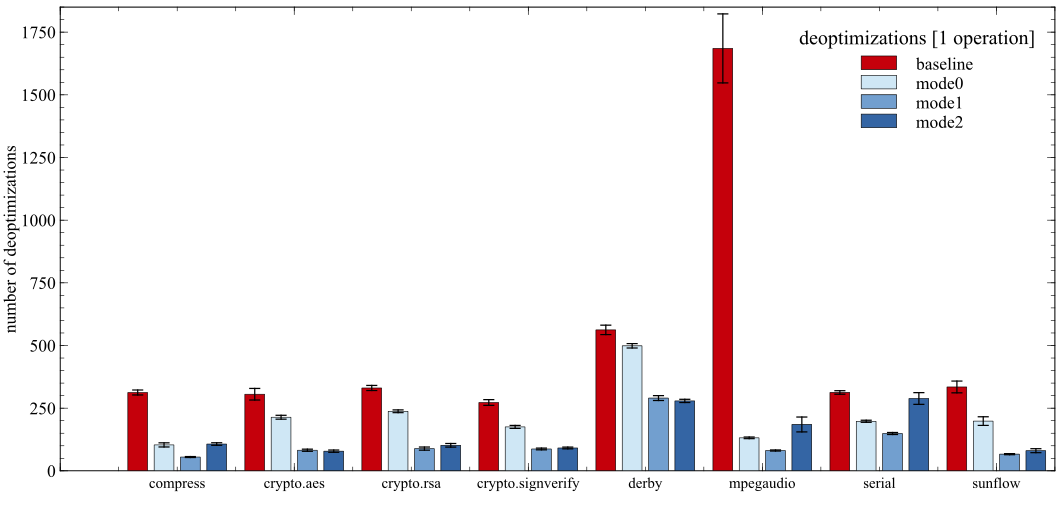
\includegraphics[width=1.0\textwidth]{figures/others_warmup_deopt.png}
    \caption{SPECjvm deoptimizations of all modes}
    \label{f:others_warmup_deopt}
  \end{center}
\end{figure}

\begin{figure}[ht]
  \begin{center}
    \centering
    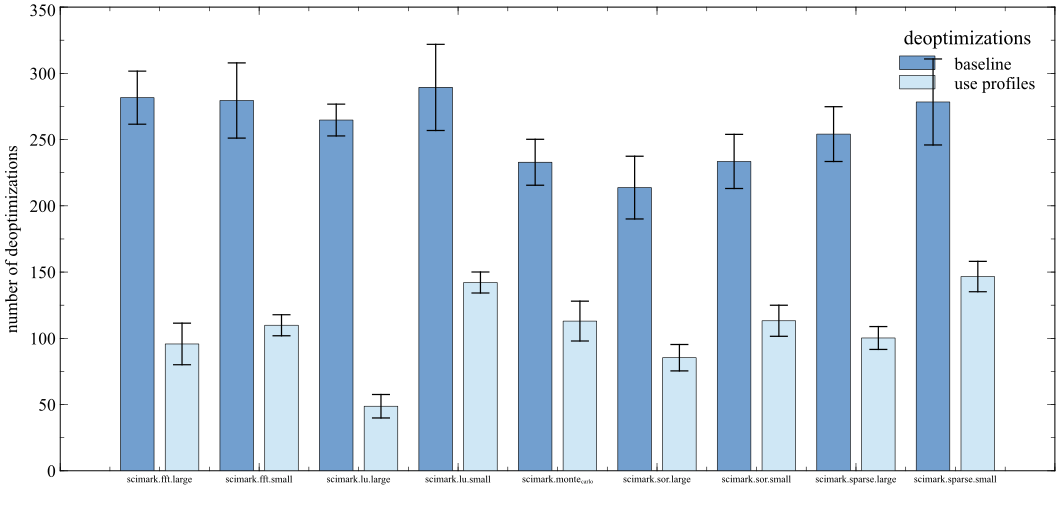
\includegraphics[width=1.0\textwidth]{figures/scimark_warmup_deopt.png}
    \caption{SPECjvm scimark deoptimizations of all modes}
    \label{f:scimark_warmup_deopt}
  \end{center}
\end{figure}

\begin{figure}[ht]
  \begin{center}
    \centering
    \includegraphics[width=1.0\textwidth]{figures/all_warmup_variation_deopt.png}
    \caption{Relative deoptimizations from baseline for all SPECjvm benchmarks}
    \label{f:all_warmup_variation_deopt}
  \end{center}
\end{figure}

\begin{figure}[ht]
  \begin{center}
    \centering
    \includegraphics[width=1.0\textwidth]{figures/octane_deopt.png}
    \caption{Octane deoptimizations of all modes} 
    \label{f:octane_deopt}
  \end{center}
\end{figure}



\begin{figure}[ht]
  \begin{center}
    \centering
    \includegraphics[width=1.0\textwidth]{figures/octane_variation_deopt.png}
    \caption{Relative deoptimizations from baseline for all Octane benchmarks}
    \label{f:octane_variation_deopt}
  \end{center}
\end{figure}

\clearpage
\section{Effect on compile queue}
\label{s:perf_compilequeue}
When designing the different CacheProfilesModes, we thought that lowering the compilation thresholds will increase the load on the compiler, especially early in program execution. This results in the compiler not being able to handle all requests immediately and the compile queue fills up. This could delay execution of compiled methods and therefore decrease performance.
\\\\
We added a new HotSpot flag \texttt{-XX:+PrintCompileQueueSize} which allows us to trace the current number of methods that are scheduled for compilation. We selected 6 indidividual benchmarks and printed their C1 and C2 compile queue for all three CacheProfileModes in Figure \ref{f:octane_queue_richards_separate_c1} to Figure \ref{f:octane_queue_deltablue_separate_c2}.
Keep in mind that the reason for the runs using cached profiles starting their compilations on later time stamps is because they need to parse the cached profile file first.
The selected benchmarks and the reason why an individual analysis was performed are listed below:
\begin{itemize}
  \item \textbf{Octane Richards:} This benchmarks achieved the highest performance benefit from using cached profiles in all three modes. We are interested to see if the compile queue load differs from worse performing benchmarks.
  \item \textbf{Octane EarleyBoyer:} This is a benchmark were \texttt{Mode 1} performs significantly better than the other two modes. Does the compile queue give as any indication why this is the case?
  \item \textbf{Octane NavierStokes:} Navierstokes has a 8\% performance increase in \texttt{Mode 2} but a 25\% performance decrease in \texttt{Mode 0} and \texttt{Mode 1}. Motivation is the same as for EarleyBoyer.
  \item \textbf{Octane Deltablue:} This benchmark achieves the highest performance loss from using cached profiles in all three modes. Together with the best benchmark (Richards) does the load on the compile queue give any indication of performance?
  \item \textbf{SPECjvm compress:} Compress is the best performing SPECjvm benchmark when using cached profiles. 
  \item \textbf{SPECjvm scimark.sparse.large:} This is the worst performing SPECjvm benchmark when using cached profiles. 
\end{itemize}
We realize that analyzing the compile queue does not really help us understanding the performance variations when using cached profiles.
The graphs showing the C1 compile queue size over time do not significantly differ, neither from the baseline, nor is there a difference between the individual modes.
The C2 compile queue graphes show different courses but we can not connect this with the benchmark performance.
\\\\
Figure \ref{f:octane_queue_richards_separate_c2} show the C2 compile queue of the Octane Richards benchmark. As expected, due to removing steps from the tiered compilation, we increased the load on C2 in \texttt{Mode 0} and \texttt{Mode 1} with compile queue peaks at around 20 scheduled compilations. Nevertheless, these modes achieve close a performance of close to 50\% better than the baseline. \texttt{Mode 2} which was designed to keep the original tiered compilation steps unmodified does not have these peaks but nevertheless achieves similar performance.
\\\\
EarleyBoyer's compile queue is displayed in Figure \ref{f:octane_queue_richards_separate_c2}. \texttt{Mode 1} performs better than the other two modes and compared to \texttt{Mode 0} seems to put even more pressure on the compile queue.
It is interesting that in this particular benchmark even the baseline version puts a lot of pressure on the compile queue early on.
\\\\
In Figure \ref{f:octane_queue_navierstokes_separate_c2} we see NavierStokes' compile queue. \texttt{Mode 2} performs best but we could not derive any indications why this is the case from looking at the queue size.
\\\\
The Deltablue benchmark shown in Figure \ref{f:octane_queue_deltablue_separate_c2} has the worst performance when using cached profiles but the compile queue size looks very similar to the one of the Richards benchmark, where performance is significantly better.
\\\\
We will omit looking at the SPECjvm benchmarks since they do not offer any new insights. The graphs can be found in the Appendix \ref{a:additional_graphs}.
\\\\
The detailed analysis of the compile queue shows that our thoughts about the effect on the compile queue were not unfounded for most of the selected benchmarks. However, we were not able to relate these influences to actual performance effects. Especially, overloading the compile queue does not necessarily negatively affect performance.
\\\\
This indicates that the performance differences are even more related to the actual code quality.
% --------------------------- Octane Richards Queue ------------------
\begin{figure}[ht]
  \begin{center}
    \centering
    \includegraphics[width=1.0\textwidth]{figures/octane_queue_richards_separate_c1.png}
    \caption{C1 Compile queue size over time Octane Richards benchmark}
    \label{f:octane_queue_richards_separate_c1}
  \end{center}
\end{figure}
\begin{figure}[ht]
  \begin{center}
    \centering
    \includegraphics[width=1.0\textwidth]{figures/octane_queue_richards_separate_c2.png}
    \caption{C2 Compile queue size over time Octane Richards benchmark}
    \label{f:octane_queue_richards_separate_c2}
  \end{center}
\end{figure}
% --------------------------- Octane EarleyBoyer Queue ------------------
\begin{figure}[ht]
  \begin{center}
    \centering
    \includegraphics[width=1.0\textwidth]{figures/octane_queue_earleyboyer_separate_c1.png}
    \caption{C1 Compile queue size over time Octane EarleyBoyer benchmark}
    \label{f:octane_queue_earleyboyer_separate_c1}
  \end{center}
\end{figure}
\begin{figure}[ht]
  \begin{center}
    \centering
    \includegraphics[width=1.0\textwidth]{figures/octane_queue_earleyboyer_separate_c2.png}
    \caption{C2 Compile queue size over time Octane EarleyBoyer benchmark}
    \label{f:octane_queue_earleyboyer_separate_c2}
  \end{center}
\end{figure}
% --------------------------- Octane NavierStokes Queue ------------------
\begin{figure}[ht]
  \begin{center}
    \centering
    \includegraphics[width=1.0\textwidth]{figures/octane_queue_navierstokes_separate_c1.png}
    \caption{C1 Compile queue size over time Octane NavierStokes benchmark}
    \label{f:octane_queue_navierstokes_separate_c1}
  \end{center}
\end{figure}
\begin{figure}[ht]
  \begin{center}
    \centering
    \includegraphics[width=1.0\textwidth]{figures/octane_queue_navierstokes_separate_c2.png}
    \caption{C2 Compile queue size over time Octane NavierStokes benchmark}
    \label{f:octane_queue_navierstokes_separate_c2}
  \end{center}
\end{figure}
% --------------------------- Octane DeltaBlue Queue ------------------
\begin{figure}[ht]
  \begin{center}
    \centering
    \includegraphics[width=1.0\textwidth]{figures/octane_queue_deltablue_separate_c1.png}
    \caption{C1 Compile queue size over time Octane Deltablue benchmark}
    \label{f:octane_queue_deltablue_separate_c1}
  \end{center}
\end{figure}
\begin{figure}[ht]
  \begin{center}
    \centering
    \includegraphics[width=1.0\textwidth]{figures/octane_queue_deltablue_separate_c2.png}
    \caption{C2 Compile queue size over time Octane Deltablue benchmark}
    \label{f:octane_queue_deltablue_separate_c2}
  \end{center}
\end{figure}
\clearpage

\section{Number and type of compilations}
\label{s:perf_compilenumber}
In this section we take a look on how cached profile modify the ratio of C1 and C2 compilations and if there is a correlation between percentage of methods using cached profiles and the resulting performance.
\\\\
We continue focusing on the 6 individual benchmarks selected in Section \ref{s:perf_compilequeue}.
We use the new HotSpot flag \texttt{-XX:+PrintCacheProfiles} that prints out the Level of each compilation and whether or not it uses cached profiles.
% --------------------------- Queue Total ------------------
\begin{figure}[ht!]
  \begin{center}
    \centering
    \includegraphics[width=1.0\textwidth]{figures/queue_total.png}
    \caption{Number of compilations for some specJVM and octane benchmarks}
    \label{f:queue_total}
  \end{center}
\end{figure}
\\
Figure \ref{f:queue_total} shows the total amount of compilations split in C1 and C2.
We see that the Octane benchmarks and the SPECjvm benchmarks behave differently. While the 4 Octane ones achieve a lower amount of C1 compilations in \texttt{Mode 0} and \texttt{Mode 1}, \texttt{Mode 2} is similar to the baseline. The two SPECjvm benchmarks have more C1 compilations in \texttt{Mode 0}, less in \texttt{Mode 1} and the same amount in \texttt{Mode 2} compared to the baseline.
\\\\
The changes in the amount of C2 compilations are very similar in all benchmarks. Using \texttt{Mode 0} and \texttt{Mode 1} results in more C2 compilations than the baseline and \texttt{Mode 2} again achieves around the same.
\\\\
If we recall the differences between the modes these results make sense. \texttt{Mode 0} lowers the thresholds of C1 compilations in case the method has a cached profile and compiles with C2 instead. This reduces the number of C1 compilations in favor of more C2 compilations. \texttt{Mode 1} does not lower the thresholds but it still promotes some C1 compilations to C2 compilations which is also seen in the numbers.
\texttt{Mode 2} leaves the tiered compilation completely untouched, we see that it also does not influence the total number of compilations significantly.
\\\\
Furthermore, we are interested how many of the compilations make use of cached profiles. Ideally, this should be 100\% but there could always me methods that have no cached profiles available because they have not been compiled when generating the profile.
Additionally, we intentionally do not use any profiles for compilation Level 1 and Level 2 as described in Section \ref{s:usingprofiles}.
The ReplayCompilation functionality does not support certain methods, e.g. lambda expressions. Since this CacheProfiles implementation is based on ReplayCompilation it will also not compile these methods using cached profiles. 
\\\\
In Figure \ref{f:richards_compilations} to Figure \ref{f:sparselarge_compilations} we show cake diagrams that visualize the portion of specific compilation types.
The results show, that the proportions are very similar if we compare different benchmarks of the same CacheProfilesMode.
\texttt{Mode 0} and \texttt{Mode 1} look similar with \texttt{Mode 1} invoking less compilations using cached profiles. 
In \texttt{Mode 2} we see Level 2 compilations appearing due to the changed tiered compilation transitions. The number of Level 3 compilations is nearly unchanged compared to \texttt{Mode 1} because these are compilations of methods where no profiles from C2 compilations are available.
The Level 2 compilations only happen if such a profile is available and usually result in another Level 4 compilation. 
% --------------------------- Compilation cake Richards ------------------
\begin{figure}[ht]
  \begin{center}
    \centering
    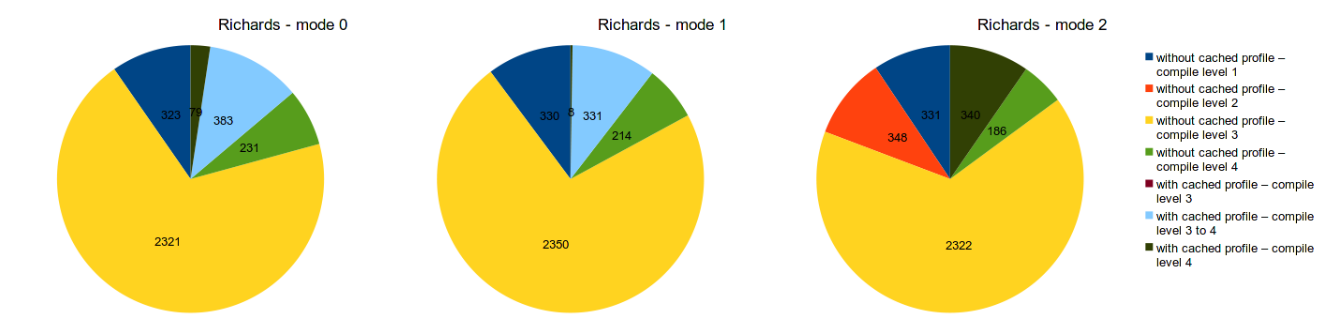
\includegraphics[width=1.0\textwidth]{figures/richards_compilations.png}
    \caption{Ratio of compilations Octane Richards benchmark}
    \label{f:richards_compilations}
  \end{center}
\end{figure}
% --------------------------- Compilation cake Richards ------------------
\begin{figure}[ht]
  \begin{center}
    \centering
    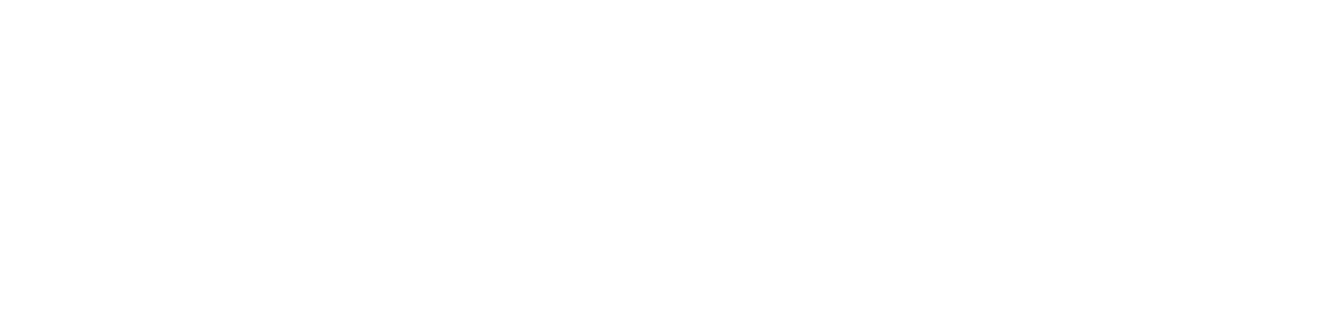
\includegraphics[width=1.0\textwidth]{figures/deltablue_compilations.png}
    \caption{Ratio of compilations Octane Deltablue benchmark}
    \label{f:deltablue_compilations}
  \end{center}
\end{figure}
% --------------------------- Compilation cake Richards ------------------
\begin{figure}[ht]
  \begin{center}
    \centering
    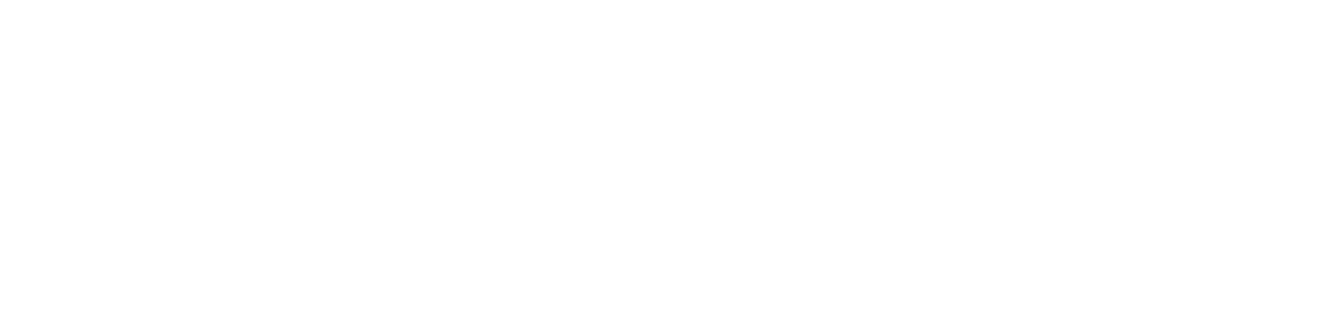
\includegraphics[width=1.0\textwidth]{figures/earleyboyer_compilations.png}
    \caption{Ratio of compilations Octane EarleyBoyer benchmark}
    \label{f:earleyboyer_compilations}
  \end{center}
\end{figure}
% --------------------------- Compilation cake Richards ------------------
\begin{figure}[ht]
  \begin{center}
    \centering
    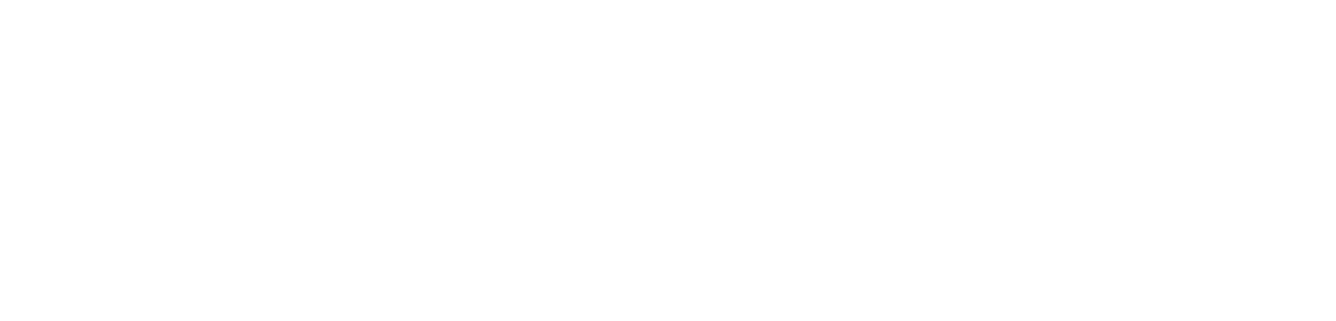
\includegraphics[width=1.0\textwidth]{figures/navierstokes_compilations.png}
    \caption{Ratio of compilations Octane NavierStokes benchmark}
    \label{f:navierstokes_compilations}
  \end{center}
\end{figure}
% --------------------------- Compilation cake compress ------------------
\begin{figure}[ht]
  \begin{center}
    \centering
    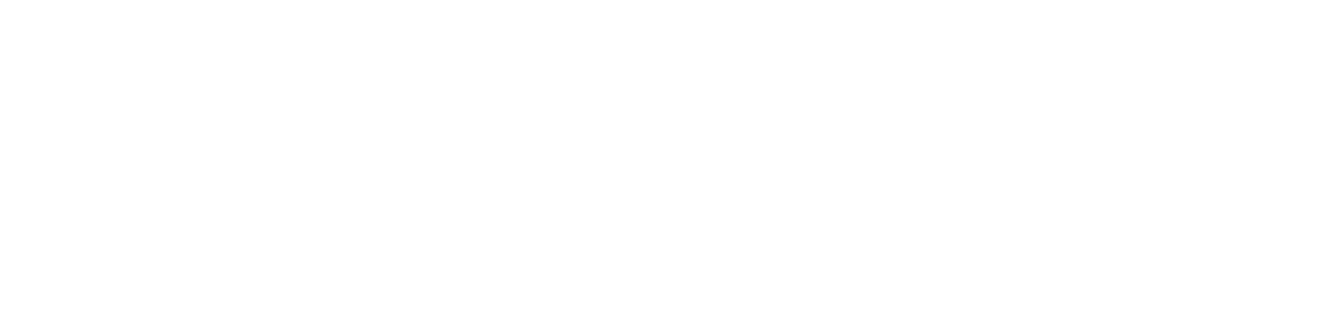
\includegraphics[width=1.0\textwidth]{figures/compress_compilations.png}
    \caption{Ratio of compilations SPECjvm compress benchmark}
    \label{f:compress_compilations}
  \end{center}
\end{figure}
% --------------------------- Compilation cake sparse.large ------------------
\begin{figure}[ht]
  \begin{center}
    \centering
    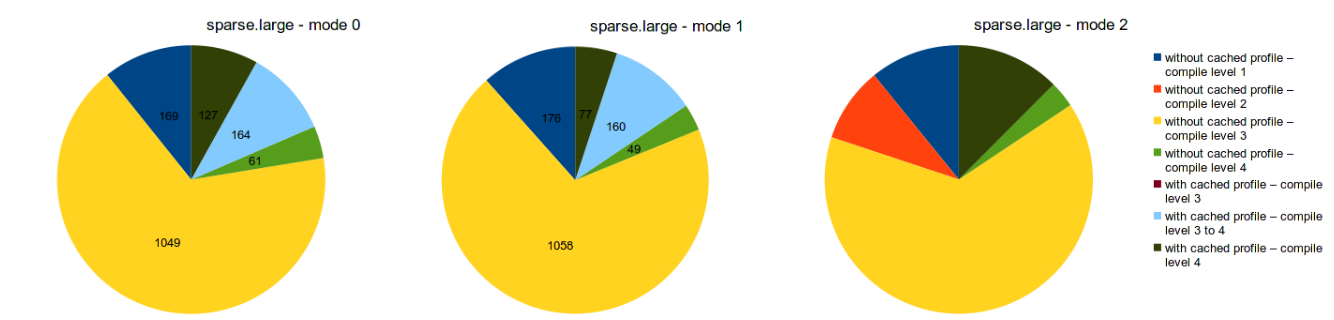
\includegraphics[width=1.0\textwidth]{figures/sparselarge_compilations.png}
    \caption{Ratio of compilations SPECjvm sparse.large benchmark}
    \label{f:sparselarge_compilations}
  \end{center}
\end{figure}
\clearpage
\section{Effect of interpreter profiles}
\label{s:perf_interpreter_profiles}
Our system makes use of two types of cached profiles. Profiles that are gathered by the interpreter and used by the C1 compiler and profiles that are gathered by a C1 compiled method and used when compiling with C2.
\\\\
We added a HotSpot flag that allows us to specify the minimum level of a compilation that dumps profiles (\texttt{-XX:DumpProfilesMinTier=}level).
Previous measurements were done using Level 3 which dumps profiles during C1 and C2 compilations.
\\\\
However, we are also interested how the system performance changes when only C2 compiler profiles are used. The system will then only use cached profiles where a C2 compilation took place in the previous profile generation run. We use the same setup as before and run the individual SPECjvm (see Figure \ref{f:others_warmup_wo_i} and Octane (see Figure \ref{f:octane_wo_i} benchmarks. 
\\\\
Most of the benchmarks do not show significantly different results compared to Section \ref{s:perf_benchmark}, where both types of cached profiles where used. There are a few benchmarks where individual modes now improve the performance while having a performance drop when using C1 and C2 profiles (e.g. NavierStokes \texttt{Mode 0}). But we also experience the other way around for example in benchmark Splay \texttt{Mode 2}. In these individual cases, we believe that for example a benchmarks C1 compilation does not profit from having cached profiles and therefore using them will even decrease performance. This happens because methods are first compiled by using cached profiles and after ten deoptimizations are compiled using generated profiles.
\\\\
The results let us conclude that the performance differences to the baseline are mostly due to the code quality of C2 compilations. Even though the number of C1 compilations is usually a lot higher than the number of C2 compilations, C2 compilations seem more crucial to the methods performance.
Since C2 is the maximum compilation level, a program might spend most of it's time in C2 compiled code.
\\\\
This again shows that it is very hard to predict JVM performance.
\begin{figure}[ht]
  \begin{center}
    \centering
    \includegraphics[width=1.0\textwidth]{figures/all_warmup_variation_wo_i.png}
    \caption{Relative performance from baseline for all SPECjvm benchmarks without using cached interpreter profiles}
    \label{f:others_warmup_wo_i}
  \end{center}
\end{figure}
\begin{figure}[ht]
  \begin{center}
    \centering
    \includegraphics[width=1.0\textwidth]{figures/octane_variation_wo_i.png}
    \caption{Relative performance from baseline for all Octane benchmarks without using cached interpreter profiles}
    \label{f:octane_wo_i}
  \end{center}
\end{figure}
\clearpage
\section{Effect of intrinsified methods}
\label{s:perf_intrinsics}
This chapter takes a quick look at the influence of method intrinsics.
The HotSpot JVM does not compile some common standard library methods. Instead it emits hand-written assembler code.
TODO
%
% \begin{figure}[ht]
%   \begin{center}
%     \centering
%     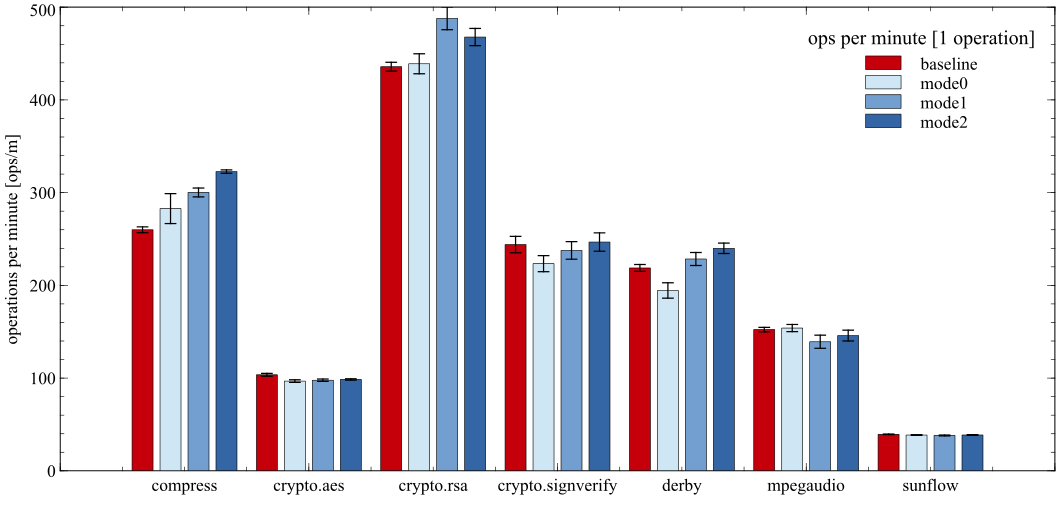
\includegraphics[width=1.0\textwidth]{figures/others_warmup_nointrinsics.png}
%     \caption{SPECjvm benchmarks on all different modes without intrinsified methods}
%     \label{f:others_warmup_nointrinsics}
%   \end{center}
% \end{figure}
%
% \begin{figure}[ht]
%   \begin{center}
%     \centering
%     \includegraphics[width=1.0\textwidth]{figures/scimark_warmup_nointrinsics.png}
%     \caption{SPECjvm scimark benchmarks on all different modes without intrinsified methods}
%     \label{f:scimark_warmup_nointrinsics}
%   \end{center}
% \end{figure}
%
%
% \begin{figure}[ht]
%   \begin{center}
%     \centering
%     \includegraphics[width=1.0\textwidth]{figures/all_warmup_nointrinsics_variation.png}
%     \caption{Relative performance from baseline for all SPECjvm benchmarks without intrinsified methods}
%     \label{f:all_warmup_nointrinsics_variation}
%   \end{center}
% \end{figure}
